\head{Ноябрь}{Листок 4. Теория чисел.}

\begin{floatingfigure}[l]{0\textwidth}
	
	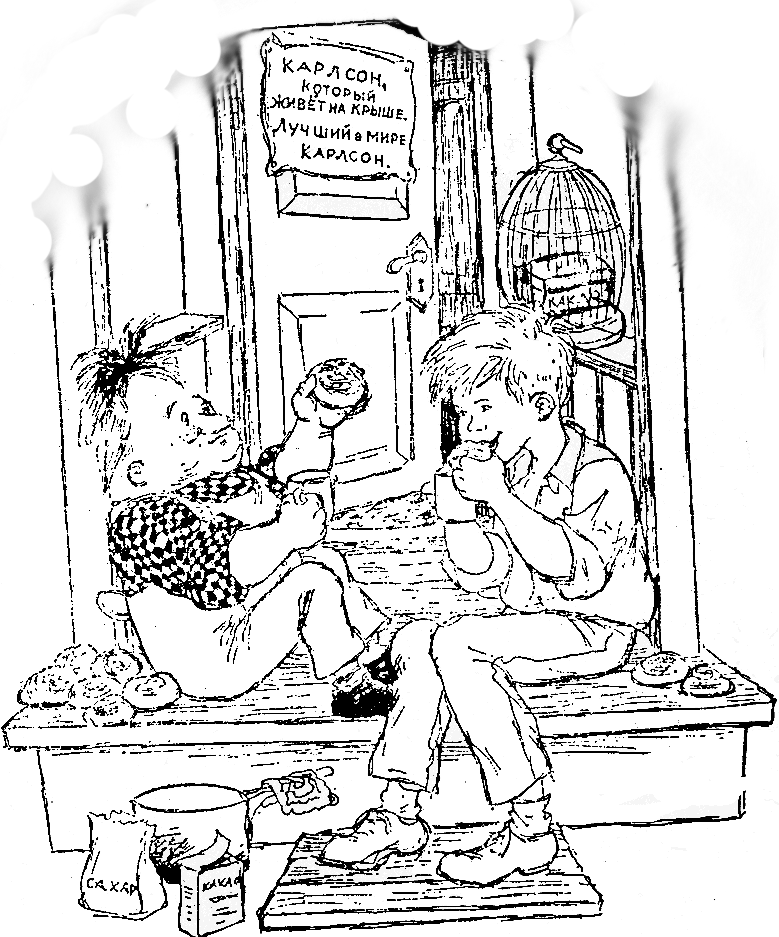
\includegraphics[scale=0.17]{./img/karlson}
\end{floatingfigure}~

\epigraph{
\textit{– Мы поделим их поровну: 7 тебе и 7 мне, – сказал Карлсон.\\
– Но так не получится, – возразил Малыш. –  7+7=14, а у нас только 10 плюшек.\\
– В нынешних школах как-то по-дурацки считают, – ответил тот. – но я из-за этого страдать не намерен. По крайней мере, свои я уже взял, – добавил он и прикрыл пухлой ладошкой дымящуюся горку.
}}{Астрид Линдгрен «Три повести о Малыше и Карлсоне».}


По определению целое число $а$ делится на не равное нулю целое число $b$, если существует целое число $q$ такое, что $a = bq$. В этом случае число $a$ называется делимым, $b$ – делителем, а $q$ – частным. В дальнейшем, речь будет идти только о целых числах.

\fbox{\begin{minipage}{0.85\textwidth}
\begin{ex}
	Запишите общий вид чисел, делящихся а) на 2; б) на 17; в) на 2012.
\end{ex}
\end{minipage}}

\begin{floatingfigure}[r]{0.25\textwidth}
	
\includegraphics[scale=0.45]{./img/dog}
\end{floatingfigure}
В литературе существует несколько способов обозначить делимость:


Если целое число $a$ делится на целое число $b$, то говорят, что $a$ кратно $b$, пишут $a\del b$. Соответственно запись $a\ndel b$ означает, что $a$ не делится на $b$, или $a$ не кратно $b$. 


Наряду с такими обозначениями используются запись $b~|~a$, означающая, что $a$ делит $b$, т.е. $a$ является делителем $b$. Запись $b~\mathrlap{\backslash}|~a$, что означает, что $a$ не делит $b$, т.е. $a$ не является делителем $b$.


Делимость целых чисел обладает несколькими основными свойствами:



\fbox{\begin{minipage}{0.85\textwidth}
\begin{prop}
Если $a$ и $b$ делятся на $c$, то их сумма и произведение тоже делятся на $c$.
\end{prop}
\end{minipage}}


\begin{dok}
    Поскольку $a\del c$ и $b\del c$, то $a = cq_1$ и $b = cq_2$, где $q_1$ и $q_2$ – целые числа. Следовательно,  $a + b = c(q_1 + q_2)$ и $ab = c_2(q_1q_2)$. Что означает по определению, что $(a + b) \del c$ и $(ab) \del c$, поскольку если    $q_1$ и $q_2$ – целые числа, то их сумма и произведение также являются целыми числами. 
\end{dok}

\fbox{\begin{minipage}{0.55\textwidth}
\begin{prop}
Если $a\del c$, но $b\ndel c$, то $(ab)\del c$, и $(a + b)\ndel c$.
\end{prop}
\end{minipage}}

\begin{dok}
1) Поскольку $a\del c$, то $a = cq$, где $q$ – целое число. Следовательно, $ab = c(qb)$, т.е. $(ab)\del c$.

2) Доказательство того, что $(a + b)\ndel c$, будем проводить методом «\textit{от противного}». Предположим, что $(a + b)\del c$, тогда из доказанного выше свойства следует, что $(a + b) + (–a)\del c$,\footnote{Здесь одно из слагаемых равно $(a + b)$ , а другое $(–a)$. Вообще говоря, здесь в неявном виде используется утверждение, что «если $a$ делится на $с$, то и $(–a)$ делится на $с$». Докажите это утверждение самостоятельно!} т.е. $b\del c$, но $b \ndel c$ по условию, значит мы пришли к противоречию. Итак, наше предположение, что $(a + b)\del c$, было неверно,  следовательно, $(a + b) \ndel c$.\footnote{При доказательстве теоремы методом «\textit{от противного}» сначала допускают, что утверждение этой теоремы неверно. Затем посредством некоторых рассуждений стараются получить либо заведомо неверное утверждение, либо утверждение, противоречащее условию теоремы. При правильных рассуждениях противоречие может получиться только за счет того, что неверным было первоначальное допущение о том, что теорема неверна. Отсюда делают вывод, утверждение теоремы верно.}
\end{dok}

Пользуясь основными свойствами, решите следующие задачи:

\begin{thm}
	Докажите, что, если $a\del b$, и $b\del c$, то $a\del c$.
\end{thm}

\begin{thm}
	Пусть $a \del c$, и $b \del d$. Докажите, что $(ab) \del (cd)$.
\end{thm}

\begin{thm}
	Даны два числа $a$ и $b$ такие, что $a\del b$. Можно ли утверждать, что $a^n\del b^n$ при любом натуральном $n$?
\end{thm}

\begin{prim}
    Эти задачи входят в листок по теории чисел уровня 1.
\end{prim}

\fbox{\begin{minipage}{0.95\textwidth}
\begin{ex}
	Запишите условия предыдущих задач и свойств, используя вместо символа $\del$ символ $|$ .
\end{ex}
\end{minipage}}

\section{Деление с остатком.}

\epigraph{
\textit{Действительность никогда не делится на разум без остатка.
}}{Автор неизвестен}

Отметим на числовой оси точки, соответствующие целым числам. Пусть $b$ – некоторое натуральное (целое положительное) число. Выделим на рисунке все целые числа, кратные $b$. Они расположены на оси на равном расстоянии $b$ друг от друга (рис.1). Каждое из этих чисел имеет общий вид $bt$, где $t$ – некоторое целое число. 

\begin{floatingfigure}[l]{0.3\textwidth}
	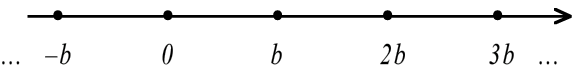
\includegraphics[scale=0.1]{./img/axis1}
\end{floatingfigure}